\chapter{Manual de Instalación.}\label{sec:ManualDeInstalacion}

\paragraph{}En este capítulo se va a explicar cómo instalar el entorno de desarrollo
para cada uno de los principales sistemas operativos. Los pasos descritos se podrán
seguir con independencia del estado previo del sistema. No se asume ningún estado previo.

\section{Consideraciones previas}

\begin{itemize}
    \item El sistema operativo y sus principales tecnologías y herramientas tienen
    como base su uso en sistemas operativos GNU/Linux, concretamente la versión 20.04 de
    la distribución de Ubuntu. Por lo que, a pesar de poder ser utilizados en cualquier
    sistema, serán en éstos donde será más fácil y óptimo su uso.

    \item Al igual que sucede en otros capítulos de este documento, se van a diferenciar
    las dos partes lógicas que componen el proyecto software: el entorno Flutter y el
    entorno Yocto.

    \item La inicaciones de este capítulo parten de sistemas con instalaciones por defecto
    y sin modificar, actualizados a la última versión disponible. Es posible que algún
    paso pueda variar, se pueda prescindir de algún paso, o que se requiera algún paso
    adicional, en función del tipo de instalación o versión.
\end{itemize}

\section{Instalación del entorno Flutter}\label{sec:entflutter}

\paragraph{}En el entorno Flutter vamos a ser capaces de desarrollar la aplicación,
pasar sus test y compilarla para diferentes plataformas.

\subsection{Instalación en sistemas operativos GNU/Linux}

\paragraph{}Para la instalación de este entorno en un sistema operativo basado en
la versión de Ubuntu 20.04 se podrá optar por 2 estrategias: correr el entorno de
forma nativa o utilizar el método basado en docker.

\subsubsection{Manera nativa:}

\paragraph{}\textbf{Nota:} Este método requiere permisos de \emph{sudo} o super usuario.

\begin{enumerate}
    \item Instalar la herramienta \textbf{\gls{git}} de control de versiones.
    \begin{lstlisting}[style=consola, numbers=left]
        $ sudo apt install git
    \end{lstlisting}

    \item Clonar el repositorio desde github
    \begin{lstlisting}[style=consola, numbers=left]
        $ git clone https://github.com/Gmatarrubia/rpi_weather.git
    \end{lstlisting}

    \item Ejecutar el script de instalación de paquetes.
    \begin{lstlisting}[style=consola, numbers=left]
        $ sudo ./installDevEnv.sh
    \end{lstlisting}

    \item Ejecutar el script de obtención de dependencias.
    \begin{lstlisting}[style=consola, numbers=left]
        $ ./getSources.sh
    \end{lstlisting}

    \item (Opcional) En caso de necesitar instalar Visual Studio Code para el desarrollo,
    se puede utilizar la siguente opctión.
    \begin{lstlisting}[style=consola, numbers=left]
        $ sudo su
        (root)$ source checkFunctions
        (root)$ check_vscode
        (root)$ exit
    \end{lstlisting}

    \item Fin de la instalación.
\end{enumerate}

\subsubsection{Entorno de desarrollo dockerizado:}

\paragraph{}\textbf{Nota:} Este método podría requerir permisos de \emph{sudo} o super
usuario.

\begin{enumerate}
    \item Instalar la herramienta \textbf{\gls{git}} de control de versiones.
    \begin{lstlisting}[style=consola, numbers=left]
        $ sudo apt install git
    \end{lstlisting}

    \item Clonar el repositorio desde github
    \begin{lstlisting}[style=consola, numbers=left]
        $ git clone https://github.com/Gmatarrubia/rpi_weather.git
    \end{lstlisting}

    \item Comprobar que el usuario pertenezca al grupo de docker, y en caso que de
    que no pertenezca al grupo, añadirlo.
    \begin{lstlisting}[style=consola, numbers=left]
        $ test $(id | grep -c docker) -eq 0 && sudo usermod -aG docker $(whoami)
    \end{lstlisting}

    \item (Opcional) En caso de necesitar instalar Visual Studio Code para el desarrollo,
    se puede utilizar la siguente opctión.
    \begin{lstlisting}[style=consola, numbers=left]
        $ sudo su
        (root)$ source checkFunctions
        (root)$ check_vscode
        (root)$ exit
    \end{lstlisting}

    \item Ejecutar el script inicialización de container. Este script construye la
    imagen en caso de que no haya sido creada previamente.
    \begin{lstlisting}[style=consola, numbers=left]
        $ ./init-docker-env.sh
    \end{lstlisting}

    \item Ejecutar el script de obtención de dependencias.
    \begin{lstlisting}[style=consola, numbers=left]
        (docker)$ ./getSources.sh
    \end{lstlisting}

    \item Fin de la instalación.
\end{enumerate}

\begin{figure}[H]
    \centering
    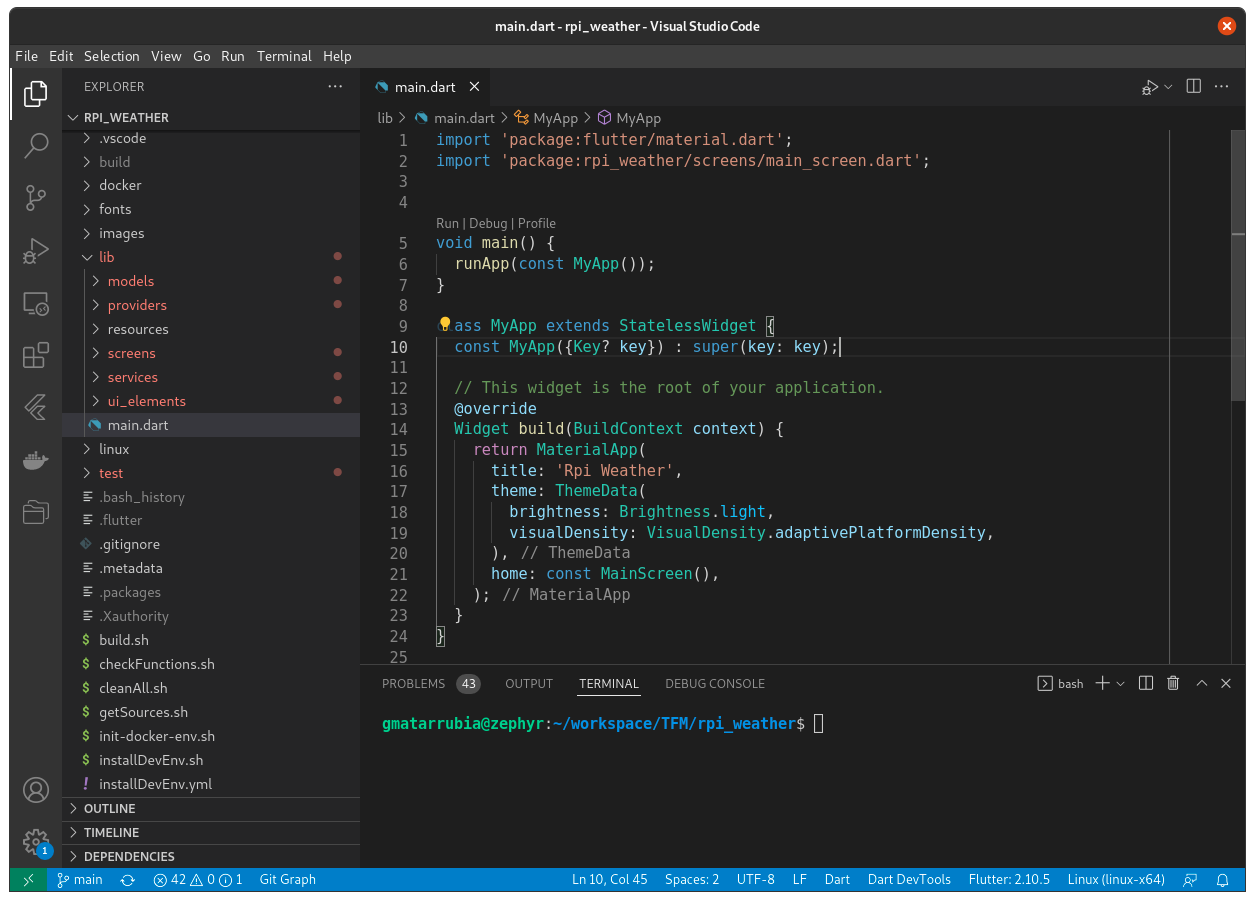
\includegraphics[width=0.95\textwidth]{imgs/vscode-ready}
	\caption[Visual Studio Code]{Visual Studio Code con el proyecto abierto.}
	\label{imgs:vscode-ready}
\end{figure}


\subsection{Instalación en sistemas operativos Windows}

\paragraph{}Tanto Visual Studio Code, como el \gls{SDK} de Flutter tienen versiones
nativas para Windows. Aunque en principio, Flutter podría trabajar indistintamente en
versiones Windows y Linux de escritorio, para evitar posibles discrepancias en la
compatibilidad de dependencias se va a trabajar dentro de un entorno Linux llamado
\gls{WSL2}. Esta característica de Windows incluida en la versión 10 y 11 en ambos
casos en la ediciones pro, permite el uso de un sistema operativo basado en el kernel
de Linux dentro del propio sistema Windows sin virtualización del hardware.

\paragraph{}\textbf{Nota:} Se requieren permisos de administrador.

\paragraph{}Por tanto los pasos para obtener nuestro entorno de desarrollo listo para
trabajar son:

\begin{enumerate}
    \item Instalar y configurar \gls{WSL2}. Para ello, abrir una consola, ya sea cmd
    o powershell, con permisos de administrador e introducir el siguiente comando:
    \begin{lstlisting}[style=cmd, numbers=left]
        wsl.exe --install
    \end{lstlisting}

    \item Reiniciar el sistema.

    \item Arrancar \gls{WSL2} desde el Menú de Inicio. Y realizar la configuración
    inicial que se nos indique, normalmente esto consiste en crear un usuario y
    contraseña.

    \item Una vez en la terminal de \gls{WSL2}, comprobamos que todo haya ido bien realizando
    la actulización de los paquetes de sistema con:
    \begin{lstlisting}[style=consola, numbers=left]
        $ sudo apt update
        $ sudo apt upgrade
    \end{lstlisting}

    \item Siguiendo en la terminal de \gls{WSL2}, instalamos la herramienta git y clonamos
    el repositorio.
    \begin{lstlisting}[style=consola, numbers=left]
        $ sudo apt install git
        $ git clone https://github.com/Gmatarrubia/rpi_weather.git
    \end{lstlisting}

    \item Instalar Visual Studio Code siguiendo la instalación recomendada en su página
    oficial: \href{https://code.visualstudio.com/download}{https://code.visualstudio.com/download}

    \item Instalar una herramienta de escritorio remoto VNC que soporte tunneling SSH.
    Recomendablemente Gsshvnc, la cual se puede descargar aquí:
    \href{https://github.com/zrax/gsshvnc/releases}{Github Gsshvnc Releases}

    \begin{figure}[H]
        \centering
        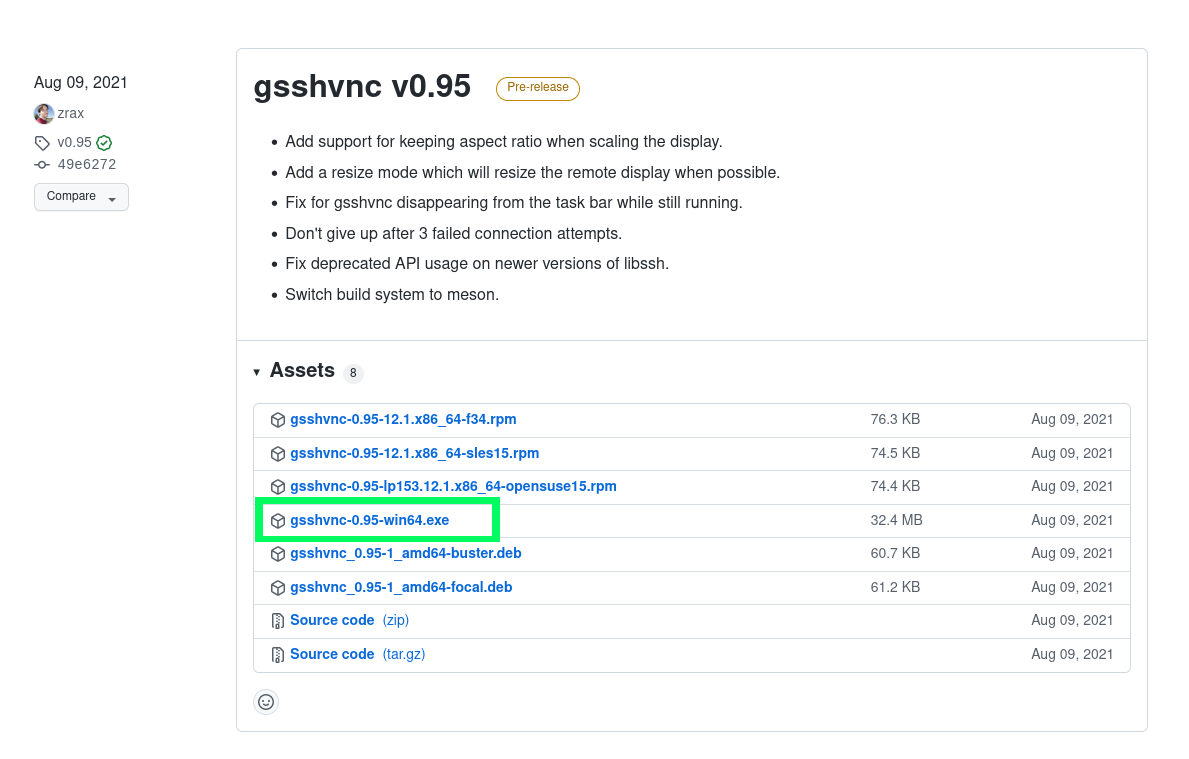
\includegraphics[width=0.95\textwidth]{imgs/gsshvnc-releases}
        \caption[gsshvnc releases]{gsshvnc página de descargas.}
        \label{imgs:gsshvnc-releases}
    \end{figure}

    \item Abrir Visual Studio Code e instalar las extensiones necesarias. Para ello
    una vez en VSCode, utilizar el atajo de teclado \emph{Ctrl+p} e introducir el siguiente
    comando. Debemos aceptar cualquier sugerencia que nos pregunte:
    \begin{lstlisting}[style=cmd]
        ext install ms-vscode-remote.remote-wsl
    \end{lstlisting}

    \item Abrir un entorno \gls{WSL2} en Visual Studio Code y abrir la carpeta del repositorio
    previamente descargado.
    blabla - insertar captura pantalla.

    \item Instalar la extension de Visual Studio Code de Flutter de la misma manera que
    en el paso anterior.
    \begin{lstlisting}[style=cmd]
        ext install Dart-Code.flutter
    \end{lstlisting}

    \item Fin de la instalación.
\end{enumerate}

\subsection{Instalación en sistemas operativos MacOS}

\paragraph{}Blabla

\newpage

\section{Instalación del entorno Yocto}

\subsection{Instalación en sistemas operativos GNU/Linux}

\paragraph{}Al igual que sucedía con el entorno de Flutter \ref{sec:entflutter}, existe
la posibilidad de correr el entorno de manera nativa o de manera \emph{dockerizada}.
Se ha diseñado una instalación similar para ambos entornos para que resulte más familiar
y por tanto más fácil de comprender. Veamos la instalación de ambos métodos:

\subsubsection{Manera nativa:}

\paragraph{}\textbf{Nota:} Este método requiere permisos de \emph{sudo} o super usuario.

\begin{enumerate}
    \item Instalar la herramienta \textbf{\gls{git}} de control de versiones.
    \begin{lstlisting}[style=consola, numbers=left]
        $ sudo apt install git
    \end{lstlisting}

    \item Clonar el repositorio desde github
    \begin{lstlisting}[style=consola, numbers=left]
        $ git clone https://github.com/Gmatarrubia/dev_env_rpi_flutter_yocto.git
    \end{lstlisting}

    \item Ejecutar el script de instalación de paquetes.
    \begin{lstlisting}[style=consola, numbers=left]
        $ cd dev_env_rpi_flutter_yocto
        $ sudo ./installDevDeps.sh
    \end{lstlisting}

    \item (Opcional) En caso de necesitar instalar Visual Studio Code para el desarrollo,
    se puede utilizar la siguente opctión.
    \begin{lstlisting}[style=consola, numbers=left]
        $ sudo su
        (root)$ source checkFunctions
        (root)$ check_vscode
        (root)$ exit
    \end{lstlisting}

    \item Fin de la instalación.
\end{enumerate}


\subsubsection{Manera basada en docker:}

\paragraph{}\textbf{Nota:} Este método requiere permisos de \emph{sudo} o super usuario
en caso que docker no se encuentre instalado.

\begin{enumerate}
    \item Instalar docker y añadir al usuario al grupo de docker.
    \begin{lstlisting}[style=consola, numbers=left]
        $ sudo apt install curl
        $ curl -fsSL https://get.docker.com -o get-docker.sh
        $ sudo sh get-docker.sh
        $ test $(id | grep -c docker) -eq 0 && sudo usermod -aG docker $(whoami)
    \end{lstlisting}

    \item Clonar el repositorio desde github
    \begin{lstlisting}[style=consola, numbers=left]
        $ git clone https://github.com/Gmatarrubia/dev_env_rpi_flutter_yocto.git
        $ cd dev_env_rpi_flutter_yocto
    \end{lstlisting}

    \item (Opcional) En caso de necesitar instalar Visual Studio Code para el desarrollo,
    se puede utilizar la siguente opctión.
    \begin{lstlisting}[style=consola, numbers=left]
        $ sudo su
        (root)$ source checkFunctions
        (root)$ check_vscode
        (root)$ exit
    \end{lstlisting}

    \item Inicializar el entorno de docker.
    \begin{lstlisting}[style=consola, numbers=left]
        $ ./init-docker-env.sh
    \end{lstlisting}

    \item Fin de la instalación.
\end{enumerate}

\begin{figure}[H]
    \centering
    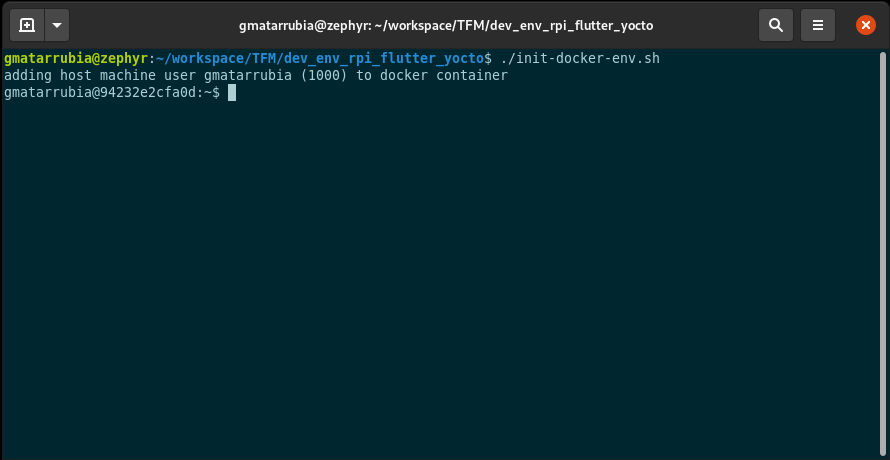
\includegraphics[width=0.95\textwidth]{imgs/yocto-docker-ready}
    \caption[yocto docker ready]{Entorno de desarrollo Yocto listo.}
    \label{imgs:yocto-docker-ready}
\end{figure}

\subsection{Instalación en sistemas operativos Windows}

\paragraph{}\textbf{Nota:} Este método es una prueba de concepto y el rendimiento puede
verse visiblemente afectado. Como opción alternativa se aconseja crear una máquina
virtual Ubunut 20.04 y seguir los consejos de la instalación en Linux de manera nativa.

\paragraph{}\textbf{Nota 2:}Se requieren permisos de administrador.

\paragraph{}Los pasos para obtener nuestro entorno de desarrollo listo para trabajar son:

\begin{enumerate}
    \item Instalar y configurar \gls{WSL2}. Para ello, abrir una consola, ya sea cmd
    o powershell, con permisos de administrador e introducir el siguiente comando:
    \begin{lstlisting}[style=cmd, numbers=left]
        wsl.exe --install
    \end{lstlisting}

    \item Reiniciar el sistema.

    \item Arrancar \gls{WSL2} desde el Menú de Inicio. Y realizar la configuración
    inicial que se nos indique, normalmente esto consiste en crear un usuario y
    contraseña.

    \item Una vez en la terminal de \gls{WSL2}, comprobamos que todo haya ido bien realizando
    la actulización de los paquetes de sistema con:
    \begin{lstlisting}[style=consola, numbers=left]
        $ sudo apt update
        $ sudo apt upgrade
    \end{lstlisting}

    \item Siguiendo en la terminal de \gls{WSL2}, instalamos la herramienta git y clonamos
    el repositorio.
    \begin{lstlisting}[style=consola, numbers=left]
        $ sudo apt install git
        $ git clone https://github.com/Gmatarrubia/dev_env_rpi_flutter_yocto.git
    \end{lstlisting}

    \item Instalar Visual Studio Code siguiendo la instalación recomendada en su página
    oficial: \href{https://code.visualstudio.com/download}{https://code.visualstudio.com/download}

    \item Abrir Visual Studio Code e instalar las extensiones necesarias. Para ello
    una vez en VSCode, utilizar el atajo de teclado \emph{Ctrl+p} e introducir el siguiente
    comando. Debemos aceptar cualquier sugerencia que nos pregunte:
    \begin{lstlisting}[style=cmd]
        ext install ms-vscode-remote.remote-wsl
    \end{lstlisting}

    \item Abrir un entorno \gls{WSL2} en Visual Studio Code y abrir la carpeta del repositorio
    previamente descargado.
    blabla - insertar captura pantalla.

    \item Ejecutar el script de instalación de paquetes.
    \begin{lstlisting}[style=consola, numbers=left]
        $ cd dev_env_rpi_flutter_yocto
        $ sudo ./installDevDeps.sh
    \end{lstlisting}

    \item Fin de la instalación.
\end{enumerate}

\subsection{Instalación en sistemas operativos MacOS}

\paragraph{}Blabla

%las referencias a artculos se ponen con \cite,
%las referencias a imgenes \ref,
%las referencias a glosario \gls,
%y las referencias a ecuaciones \eqref